\chapter{Introduction}\label{chap:introduction}

Content Delivery Networks (CDNs) are responsible for the largest share of traffic in the Internet \cite{}.
CDNs distribute popular contant to caches in many geographical areas to save bandwidth by avoiding unnecessary multihop retransmission \cite{}.
By bringing the content geographically closer to the user, CDNs also reduce the latency of the services.
TODO The exploitation of web caching and the invention of CDNs resolved the challenge of networks congestion.
The growing

Stakeholders
end user / content providers
content delivery network operators
Internet Service Providers

However, in today's Internet the inter-ISP traffic routing is based on a complex topology defined by inter-ISP relationships, e.g., peering or customer-to-provider, and ISP classifications such as \tier, large and small ISPs, and stub ISPs. Hence, these economic relations play an important role in the actual Internet traffic flow. However, this topology of the Internet is not taken into account by most evaluations of P2P guidance approaches, which limits the practical relevance of the results. Furthermore, it is an open question how much BitTorrent traffic is located in which region of the Internet. However, this is a prerequisite in order to estimate the potential of ALTO mechanisms.
Therefore in this thesis, we model

In today's Internet new challenges arise in mobile networks.
Mobile traffic growth due to
High definition video content, higher resolution displays
Higher number of mobile devices
Mobile live streaming and broadcasting services
steep increase in mobile traffic \cite{} which is expected to reach by 2018 roughly 60\% of total network traffic, the majority of which will be video.
The next generation of 5G mobile networks prepares for 1000 times data challenge.
Higher access rates and increased densification of the network infrasturcture.

With the explosion of access rates and number of base stations the backhaul of wireless networks will also become congested \cite{}.
To reduce the load on the backhaul the research community suggests to install caches in gateway routers between the wireless network and the Internet (e.g. in 4G this is called S-GW), in base stations of different sizes (small or regular size cells), and in end-user devices.
A recent approach \cite{valancius2009greening} proposes to augment spare capacities on customer premise equipment (CPE) such as home gateways or nano data-centers (NaDas) to assist content delivery, showing that there is a high potential to save energy, although the capacity of home gateways is small and the uplink is limited.
The content is transported in a peer-to-peer manner keeping the traffic within the autonomous system (AS).
The caches are organized in a hierarchy, where caches in the lowest tier are requested first and the request is forwarded to the next tier, if the requested object is not found.
Another example for a hierarchical caching system with bandwidth constraints are femto caching architectures \cite{golrezaei2013femtocaching}, where content is cached on femto-basestations with small capacity but with considerable storage space.
The potential of these approaches highly depends on the number of caches available and their capacity for content delivery.
%Our goal is to assess the potential of content delivery networks using a high number of caches with limited capacity.

The performance of hierarchical cache networks can be accurately determined by analytic models developed in recent work \cite{che2002hierarchical, martina2014unified}.
The models do not consider constraints that limit the capability of caches to upload content such as the bandwidth of the uplink.
%In the NaDa approach the upload bandwidth of caches is limited.
Therefore, in this thesis the upload bandwidth the system is modeled as loss network consisting of a server for each of the caches, to consider the limited upload bandwidth.

To further increase the overall backhaul capacity current concepts such as BeWifi\footnote{\url{http://www.bewifi.es/}} also consider multiple connections to the Internet, thereby sharing and aggregating available backhaul access link capacities.
The question is which sharing policy to apply for which system characteristics.
In the case of BeWifi, which considers access link sharing among neighboring users, each user should only share its access link when having spare capacity in order to avoid negatively affecting his own Internet connections.
%Therefore, two thresholds were introduced, i) a support threshold until which utilization a user will offer bandwidth to other users, and ii) an offloading threshold indicating from which utilization a user can offload to supporting neighbors.
It is hard and non-intuitive to determine the threshold settings for fair and effective operation of a bandwidth sharing system.
Therefore in this thesis a partial bandwidth sharing environment with offloading policy is investigated using an analytic model.
A direct application of the model is the aggregation of backhaul bandwidth by connecting neighboring access links.

The objectives of this monograph can be summarized as follows.
The first goal is to provide a thourough understaning of the nature of today's content delivery networks and their distirbution of resources on AS level.
This knowledge allows to assess the costs produced by current content delivery approaches and estimate their optimization potential.
Furthermore, we use this knowledge to ...
The second goal is to analyze the performance of hierachical cache networks with limited capacity in order to assess their potential to support content delivery.
The final objective is to evaluate the performance of bandwidth aggregation systems in heterogeneous load conditions.

A detailed description of the scientific contribution in this monograph is given in the following.

%\section{Scope of Considered Stakeholders}\label{sec:introduction:considered_stakeholders}
\newpage
\section{Scientific Contribution}\label{sec:introduction:scientific_contribution}

This section summarizes the contribution of this monograph to the field of hierarchical content delivery networks and the potential to

\begin{figure}
\centering
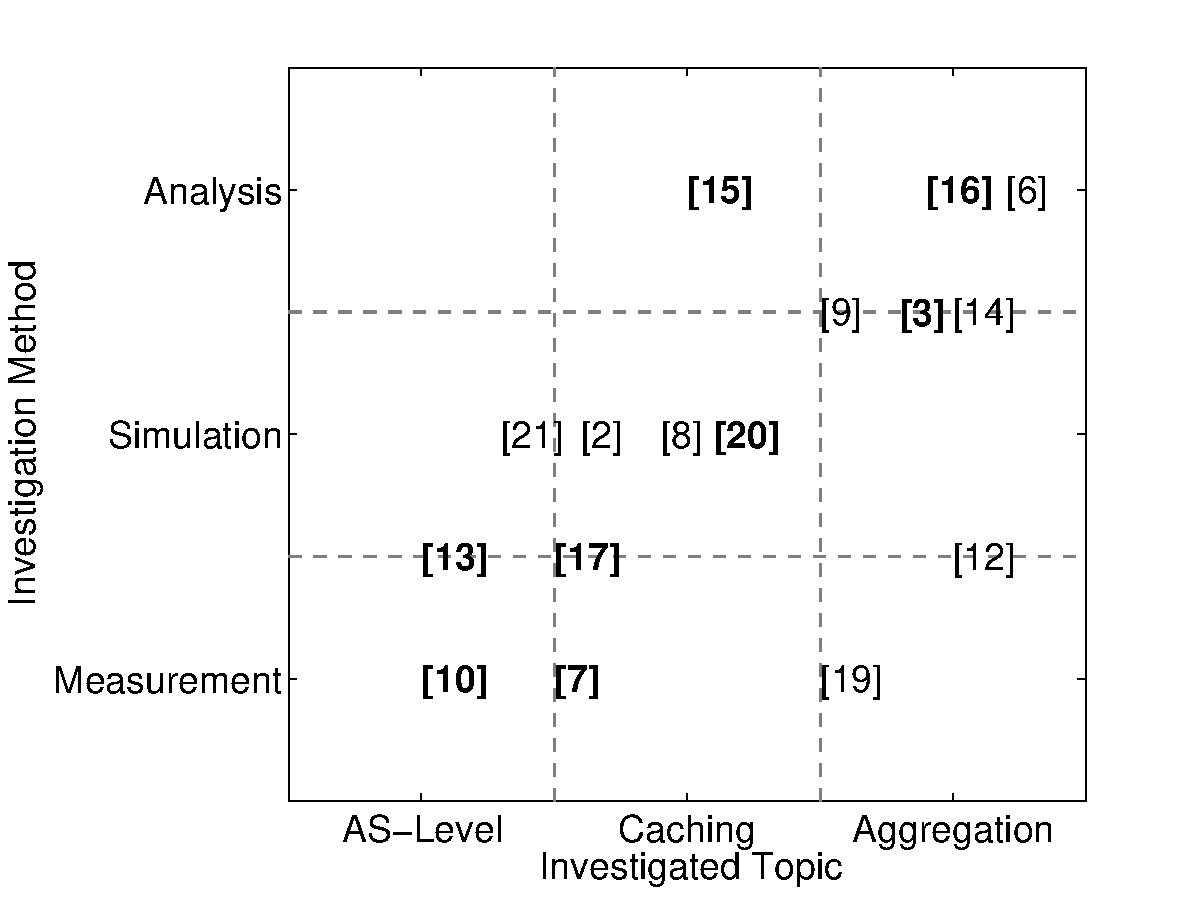
\includegraphics{figures/publications}
\caption{Contribution of this work as a classification of the research studies conducted by the author.}\label{fig:introduction:publications}
\end{figure}

In \reffig{fig:introduction:publications} we classify the areas of research as well as scientific methods used in relation to the chapters of this monograph.
The x-axis shows the impacted areas of research, i.e. topics related to the mobile network, the application domain or cloud technologies.
The y-axis details the applied scientific method.
In the theoretical area methods from queueing theory, mean value analysis and the analysis of random variables are used.
Measurements were performed using testbeds and custom software tools.
Simulation studies, performed using \gls{DES}, and created analysis tools are summarised in the practical area.

Annotations are used to highlight scientific publication whose content contributes to the respective chapters.

The first contribution of this monograph is a discussion of the impact of
We study the impact of , and investigate the potential of network parameter optimisation as a means to .

As a second contribution, we provide models for
The models do not consider constraints that limit the capability of caches to upload content such as the bandwidth of the uplink.
%In the NaDa approach the upload bandwidth of caches is limited.
To consider the upload bandwidth the system is modeled as loss network consisting of a server for each of the caches. The exact stationary distribution of the loss network is too complex to evaluate.
In \cite{tan2013optimal} the system is analyzed under large system asymptotic where simplifications occur.
We use a different approach by approximating the arrival rate of requests at the caches.
This allows us to effectively assess the loss probability by using a simple form of the Erlang formula for a loss network.
Even for traffic with highly heterogeneous request rates the approximation reflects the system performance.
We show that the streaming mechanism allows
However, further study shows that in fact
Furthermore, we provide
TODO REPHRASE: During off-peak operation of the network, the users can cheaply populate their caches with parts of popular contents.

As a third contribution, we discuss the
To this end, we study the performance of
We derive guidelines for
Furthermore, we discuss a mechanism to
Finally, we present a mechanism to

\section{Outline of Thesis}\label{sec:introduction:outline}

In \refchap{chap:aslevel} we study
First,
Then,
Finally,

\refchap{chap:hierarchical} focuses on
For Video Streaming, we study the impact
To address the second scenario, we discuss

In \refchap{chap:aggregation} we study
First,
Then,
We analyse traffic characteristics and use them as input for a simulation model
Combining these results, we evaluate the impact of different virtual server configurations and scaling strategies.
Finally, we consider resource allocation

In \refchap{chap:conclusion} we provide a summary of the major contributions of this work and suggest future potential research directions.
